\documentclass[11pt,a4paper]{report}
\usepackage[textwidth=37em,vmargin=30mm]{geometry}
\usepackage{calc,xunicode,amsmath,amssymb,paralist,enumitem,tabu,booktabs,datetime2,xeCJK,xeCJKfntef,listings}
\usepackage{tocloft,fancyhdr,tcolorbox,xcolor,graphicx,eso-pic,xltxtra,xelatexemoji}

\newcommand{\envyear}[0]{2024}
\newcommand{\envdatestr}[0]{2024-10-13}
\newcommand{\envfinaldir}[0]{webdb/2024/20241013/final}

\usepackage[hidelinks]{hyperref}
\hypersetup{
    colorlinks=false,
    pdfpagemode=FullScreen,
    pdftitle={Web Digest - \envdatestr}
}

\setlength{\cftbeforechapskip}{10pt}
\renewcommand{\cftchapfont}{\rmfamily\bfseries\large\raggedright}
\setlength{\cftbeforesecskip}{2pt}
\renewcommand{\cftsecfont}{\sffamily\small\raggedright}

\setdefaultleftmargin{2em}{2em}{1em}{1em}{1em}{1em}

\usepackage{xeCJK,xeCJKfntef}
\xeCJKsetup{PunctStyle=plain,RubberPunctSkip=false,CJKglue=\strut\hskip 0pt plus 0.1em minus 0.05em,CJKecglue=\strut\hskip 0.22em plus 0.2em}
\XeTeXlinebreaklocale "zh"
\XeTeXlinebreakskip = 0pt


\setmainfont{Brygada 1918}
\setromanfont{Brygada 1918}
\setsansfont{IBM Plex Sans}
\setmonofont{JetBrains Mono NL}
\setCJKmainfont{Noto Serif CJK SC}
\setCJKromanfont{Noto Serif CJK SC}
\setCJKsansfont{Noto Sans CJK SC}
\setCJKmonofont{Noto Sans CJK SC}

\setlength{\parindent}{0pt}
\setlength{\parskip}{8pt}
\linespread{1.15}

\lstset{
	basicstyle=\ttfamily\footnotesize,
	numbersep=5pt,
	backgroundcolor=\color{black!5},
	showspaces=false,
	showstringspaces=false,
	showtabs=false,
	tabsize=2,
	captionpos=b,
	breaklines=true,
	breakatwhitespace=true,
	breakautoindent=true,
	linewidth=\textwidth
}






\newcommand{\coverpic}[2]{
    % argv: itemurl, authorname
    Cover photo by #2~~(\href{#1}{#1})
}
\newcommand{\makeheader}[0]{
    \begin{titlepage}
        % \newgeometry{hmargin=15mm,tmargin=21mm,bmargin=12mm}
        \begin{center}
            
            \rmfamily\scshape
            \fontspec{BaskervilleF}
            \fontspec{Old Standard}
            \fontsize{59pt}{70pt}\selectfont
            WEB\hfill DIGEST
            
            \vfill
            % \vskip 30pt
            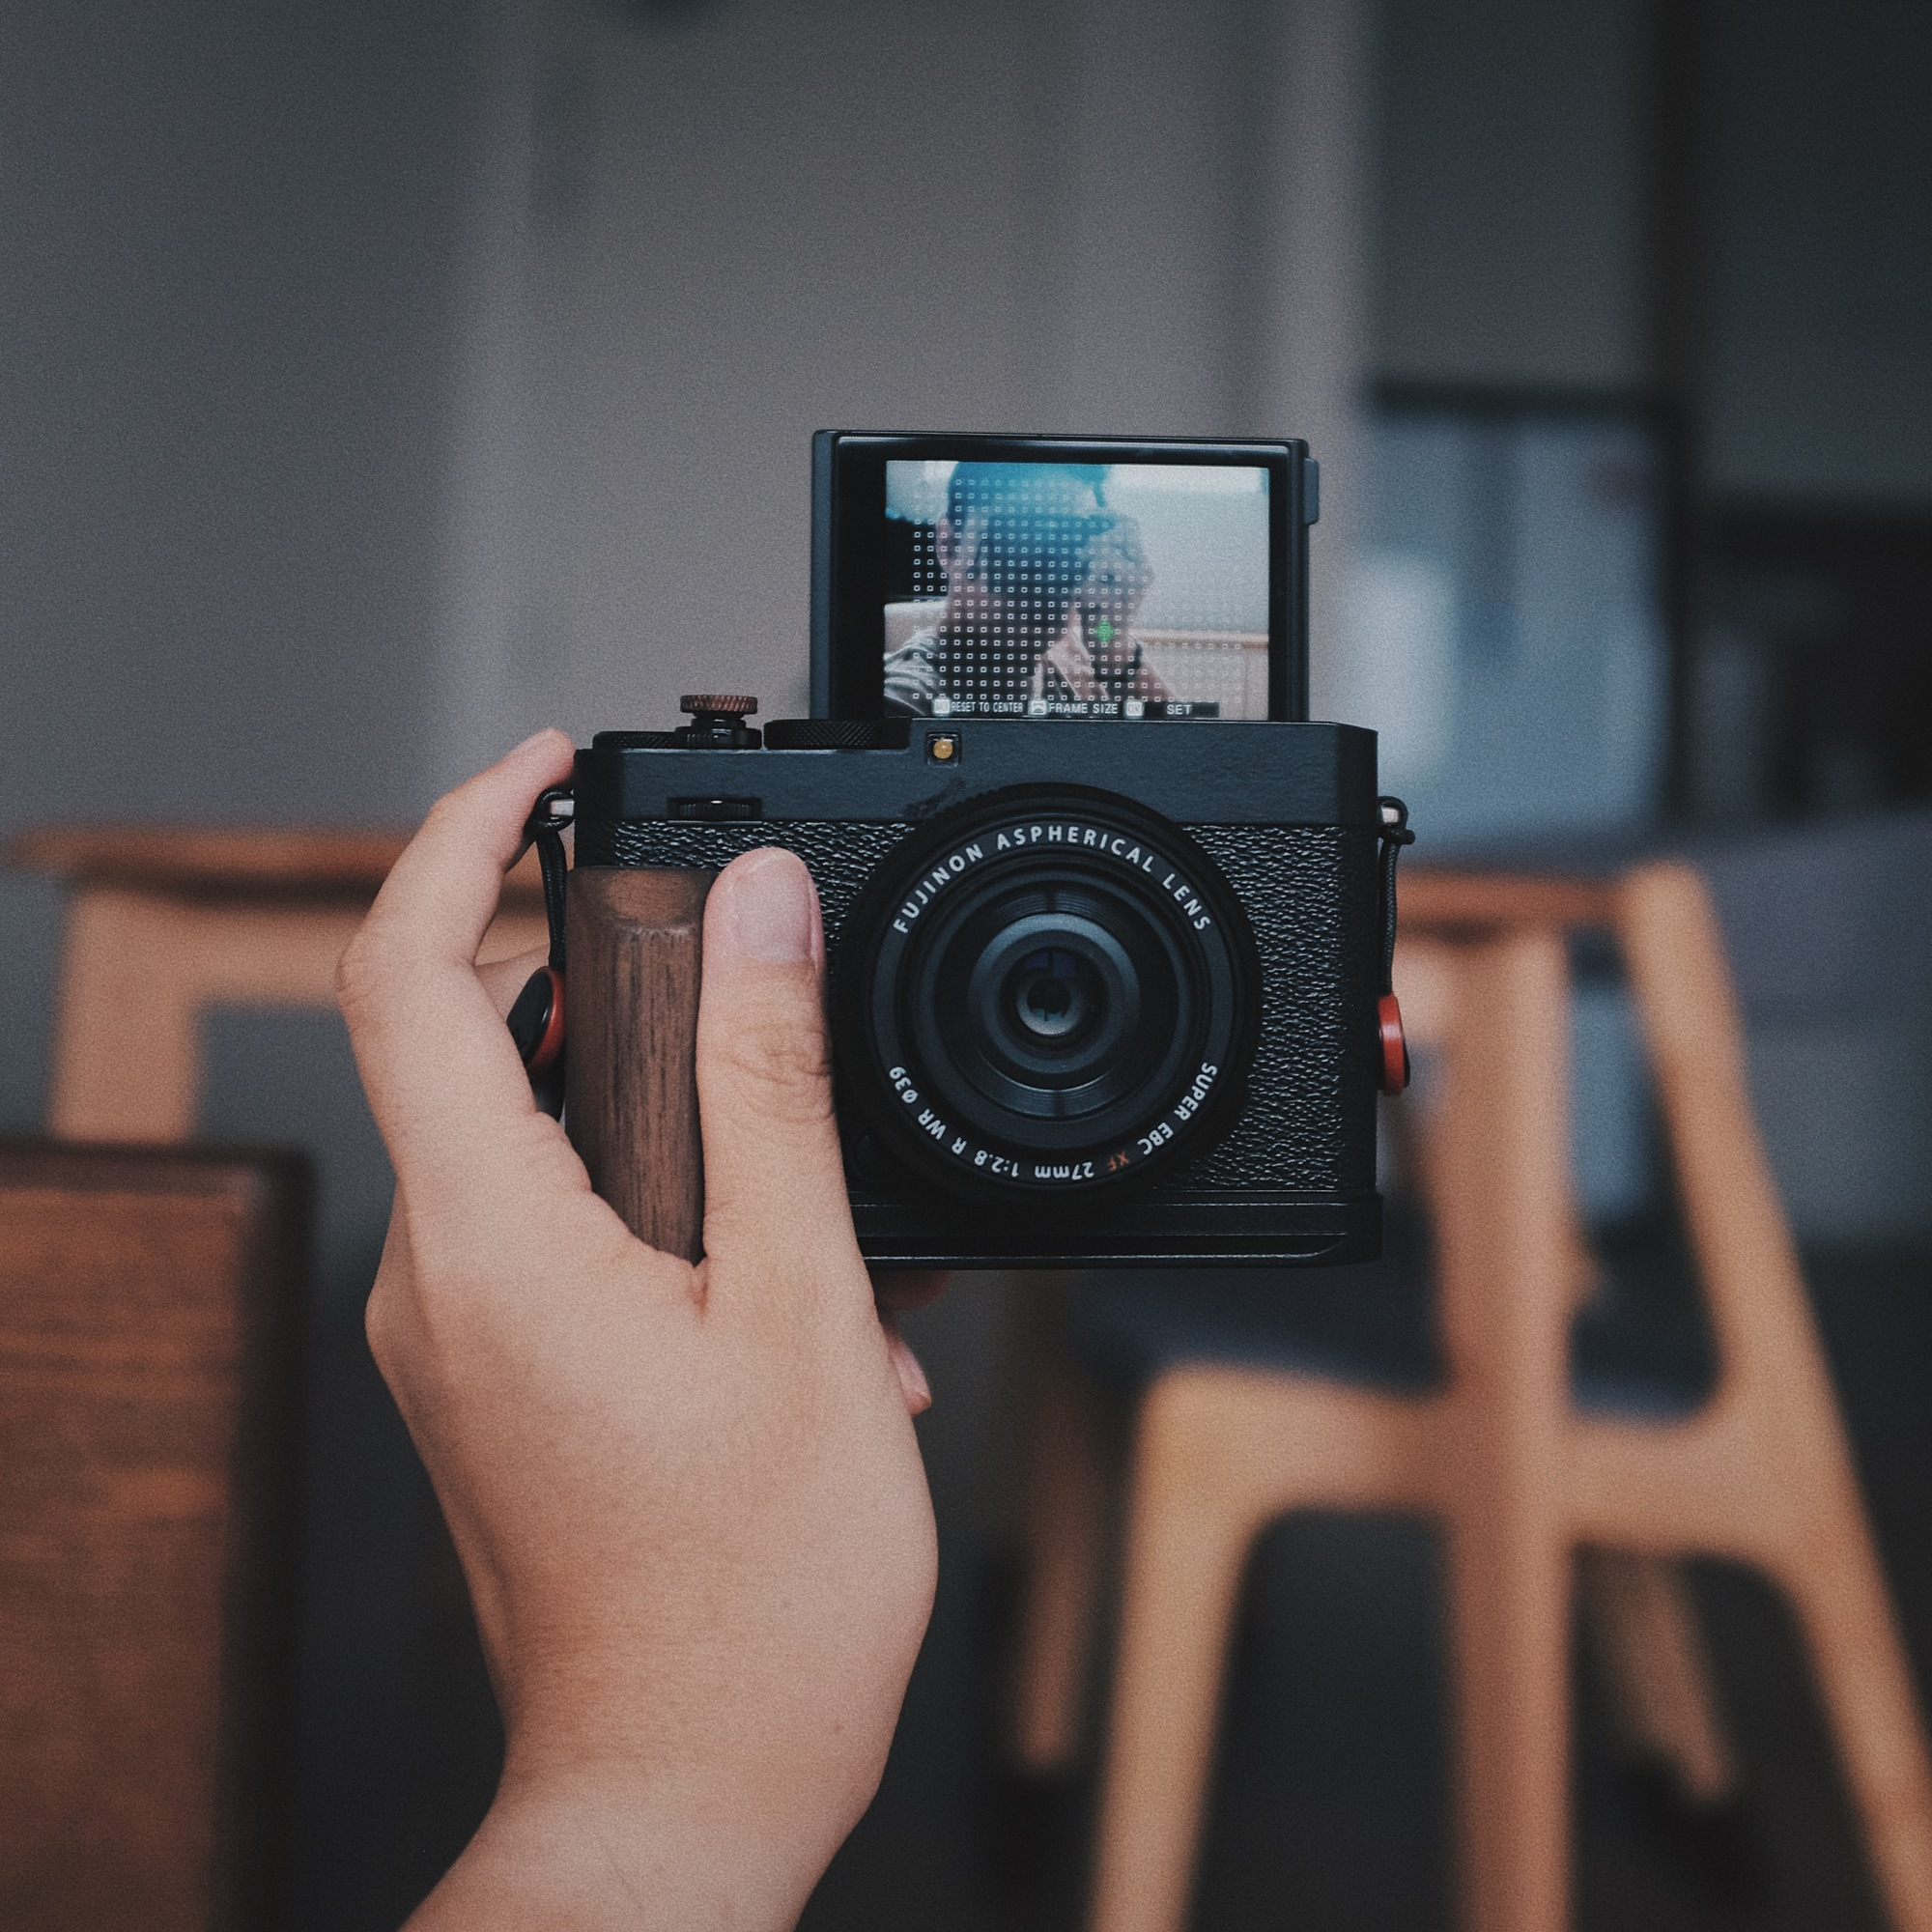
\includegraphics[width=\linewidth]{\envfinaldir/coverpic-prod.jpg}\par
            % \vskip 30pt
            \vfill

            \normalsize\rmfamily\scshape
            \copyright{} The Web Digest Project \hfill\large \envdatestr
        \end{center}
    \end{titlepage}
    % \restoregeometry
}
\newcommand{\simplehref}[1]{%
    \textcolor{blue!80!green}{\href{#1}{#1}}%
}
\renewcommand{\contentsname}{\center\Huge\sffamily\bfseries Contents\par\vskip 20pt}
\newcounter{ipartcounter}
\setcounter{ipartcounter}{0}
\newcommand{\ipart}[1]{
    % \vskip 20pt
    \clearpage
    \stepcounter{ipartcounter}
    \phantomsection
    \addcontentsline{toc}{chapter}{#1}
    % \begin{center}
    %     \Huge
    %     \sffamily\bfseries
    %     #1
    % \end{center}
    % \vskip 20pt plus 7pt
}
\newcounter{ichaptercounter}
\setcounter{ichaptercounter}{0}
\newcommand{\ichapter}[1]{
    % \vskip 20pt
    \clearpage
    \stepcounter{ichaptercounter}
    \phantomsection
    \addcontentsline{toc}{section}{\numberline{\arabic{ichaptercounter}}#1}
    \begin{center}
        \Huge
        \sffamily\bfseries
        #1
    \end{center}
    \vskip 20pt plus 7pt
}
\newcommand{\entrytitlefont}[1]{\subsection*{\raggedright\Large\sffamily\bfseries#1}}
\newcommand{\entryitemGeneric}[2]{
    % argv: title, url
    \parbox{\linewidth}{
        \entrytitlefont{#1}\par\vskip 5pt
        \footnotesize\ttfamily\mdseries
        \simplehref{#2}
    }\vskip 11pt plus 11pt minus 1pt
}
\newcommand{\entryitemGithub}[3]{
    % argv: title, url, desc
    \parbox{\linewidth}{
        \entrytitlefont{#1}\par\vskip 5pt
        \footnotesize\ttfamily\mdseries
        \simplehref{#2}\par\vskip 5pt
        \small\rmfamily\mdseries#3
    }\vskip 11pt plus 11pt minus 1pt
}
\newcommand{\entryitemAp}[3]{
    % argv: title, url, desc
    \parbox{\linewidth}{
        \entrytitlefont{#1}\par\vskip 5pt
        \footnotesize\ttfamily\mdseries
        \simplehref{#2}\par\vskip 5pt
        \small\rmfamily\mdseries#3
    }\vskip 11pt plus 11pt minus 1pt
}
\newcommand{\entryitemHackernews}[3]{
    % argv: title, hnurl, rawurl
    % \parbox{\linewidth}{
    %     \entrytitlefont{#1}\par\vskip 5pt
    %     \footnotesize\ttfamily\mdseries
    %     \simplehref{#3}\par
    %     \textcolor{black!50}{\href{#2}{#2}}
    % }\vskip 11pt plus 11pt minus 1pt
    \begin{minipage}{\linewidth}
            \entrytitlefont{#1}\par\vskip 5pt
            \footnotesize\ttfamily\mdseries
            \simplehref{#3}\par
            \textcolor{black!50}{\href{#2}{#2}}
    \end{minipage}\par\vskip 11pt plus 11pt minus 1pt
}







\begin{document}

\makeheader

\tableofcontents\clearpage




\ipart{Developers}
\ichapter{Hacker News}
\entryitemTwoLinks{PayPal (USA) will automatically share data about you to participating stores}{https://news.ycombinator.com/item?id=41822178}{https://www.paypal.com/us/legalhub/upcoming-policies-full}

\entryitemTwoLinks{The ACF plugin on the WordPress directory has been taken over by WordPress.org}{https://news.ycombinator.com/item?id=41821400}{https://twitter.com/wp\_acf/status/1845169499064107049}

\entryitemTwoLinks{Exploring Typst, a new typesetting system similar to LaTeX}{https://news.ycombinator.com/item?id=41821361}{https://blog.jreyesr.com/posts/typst/}

\entryitemTwoLinks{Secure Custom Fields by WordPress.org}{https://news.ycombinator.com/item?id=41821336}{https://wordpress.org/plugins/advanced-custom-fields/}

\entryitemTwoLinks{Starship Flight 5 license issued by FAA}{https://news.ycombinator.com/item?id=41820785}{https://drs.faa.gov/browse/excelExternalWindow/DRSDOCID173891218620231102140506.0001?modalOpened=true}

\entryitemTwoLinks{Germany's 49-euro ticket resulted in significant shift from road to rail}{https://news.ycombinator.com/item?id=41819481}{https://www.mcc-berlin.net/en/news/information/information-detail/article/49-euro-ticket-resulted-in-significant-modal-shift-from-road-to-rail.html}

\entryitemTwoLinks{The phone ban has had a big impact on school work}{https://news.ycombinator.com/item?id=41819442}{https://icelandmonitor.mbl.is/news/news/2024/10/09/the\_phone\_ban\_has\_had\_a\_big\_impact\_on\_school\_work/}

\entryitemTwoLinks{Windows 11 24H2 hoards 8.63 GB of junk you can't delete}{https://news.ycombinator.com/item?id=41818815}{https://www.theregister.com/2024/10/11/windows\_update\_cleanup/}

\entryitemTwoLinks{How I animate 3Blue1Brown [video]}{https://news.ycombinator.com/item?id=41818779}{https://www.youtube.com/watch?v=rbu7Zu5X1zI}

\entryitemTwoLinks{Six transplant patients in Brazil contract HIV from infected organs}{https://news.ycombinator.com/item?id=41818775}{https://www.reuters.com/world/americas/six-transplant-patients-brazil-contract-hiv-infected-organs-2024-10-11/}

\entryitemTwoLinks{FreeBSD: How Can We Make It More Attractive to New Users?}{https://news.ycombinator.com/item?id=41818595}{https://gyptazy.com/freebsd-how-can-we-make-it-more-attractive-to-new-users/}

\entryitemTwoLinks{1 bug, \$50k in bounties, a Zendesk backdoor}{https://news.ycombinator.com/item?id=41818459}{https://gist.github.com/hackermondev/68ec8ed145fcee49d2f5e2b9d2cf2e52}

\entryitemTwoLinks{PostgreSQL Streaming Replication (WAL); What It Is and How to Configure One}{https://news.ycombinator.com/item?id=41818446}{https://mindhub365.com/sql/postgresql-streaming-replication-wal-what-it-is-and-how-to-configure-one/}

\entryitemTwoLinks{Psilocybin bests SSRI for major depression in first long-term comparison}{https://news.ycombinator.com/item?id=41818420}{https://www.medscape.com/viewarticle/psilocybin-bests-ssri-major-depression-first-long-term-2024a1000h77}

\entryitemTwoLinks{DuckStation}{https://news.ycombinator.com/item?id=41818057}{https://github.com/stenzek/duckstation}

\entryitemTwoLinks{Google is preparing to let you run Linux apps on Android, just like Chrome OS}{https://news.ycombinator.com/item?id=41816756}{https://www.androidauthority.com/android-linux-terminal-app-3489887/}

\entryitemTwoLinks{My WordPress Slack Ban}{https://news.ycombinator.com/item?id=41815614}{https://linuxjedi.co.uk/my-wordpress-slack-ban/}

\entryitemTwoLinks{AMD's Turin: 5th Gen EPYC Launched}{https://news.ycombinator.com/item?id=41815268}{https://chipsandcheese.com/p/amds-turin-5th-gen-epyc-launched}

\entryitemTwoLinks{Swarm, a new agent framework by OpenAI}{https://news.ycombinator.com/item?id=41815173}{https://github.com/openai/swarm}

\entryitemTwoLinks{An exoskeleton let a paralyzed man walk, then its maker refused repairs}{https://news.ycombinator.com/item?id=41813720}{https://www.washingtonpost.com/nation/2024/10/08/exoskeleton-paralyzed-repairs-michael-straight/}\ichapter{Phoronix}
\entryitemGeneric{\hskip 0pt{}Wayland Protocols 1.38 Brings System Bell, FIFO \& Commit Timing Protocols}{https://www.phoronix.com/news/Wayland-Protocols-1.38}

\entryitemGeneric{\hskip 0pt{}AMD XDNA Linux Driver Updated As It Nears The Upstream Kernel}{https://www.phoronix.com/news/AMD-XDNA-Linux-Driver-v4}

\entryitemGeneric{\hskip 0pt{}BeOS-Inspired Haiku Enabling More Intel Hardware \& Driving Kernel Optimizations}{https://www.phoronix.com/news/Haiku-OS-September-2024}

\entryitemGeneric{\hskip 0pt{}Intel Panther Lake H EDAC Support Posted For Linux}{https://www.phoronix.com/news/Intel-Panther-Lake-EDAC-Linux}

\entryitemGeneric{\hskip 0pt{}AMD Job Posting Confirms More Details Around Their AI GPU Compute Stack Plans}{https://www.phoronix.com/news/AMD-GPU-AI-Stack-Job-Details}

\entryitemGeneric{\hskip 0pt{}KDE Developers Fixing Initial Bugs From Plasma 6.2}{https://www.phoronix.com/news/KDE-Plasma-6.2-Fixing-Bugs}

\entryitemGeneric{\hskip 0pt{}AMD To Integrate "Project Caliptra" Into Products Beginning In 2026}{https://www.phoronix.com/news/AMD-Project-Caliptra-2026}

\entryitemGeneric{\hskip 0pt{}Arm Exploring IO\_uring For Graphics Drivers For Better Performance \& Synchronization}{https://www.phoronix.com/news/DRM-Graphics-Drivers-IO\_uring}

\entryitemGeneric{\hskip 0pt{}AVX-512 Performance With 256-bit vs. 512-bit Data Path For AMD EPYC 9005 CPUs}{https://www.phoronix.com/review/amd-epyc-9755-avx512}


\ipart{Developers~~~~(zh-Hans)}
\ichapter{Solidot}
\entryitemGeneric{\hskip 0pt{}男子通过苹果 AI 的短信总结获悉分手的消息}{https://www.solidot.org/story?sid=79473}

\entryitemGeneric{\hskip 0pt{}苹果研究员发现大模型不能形式推理}{https://www.solidot.org/story?sid=79472}

\entryitemGeneric{\hskip 0pt{}Google 准备让用户在 Android 上运行 Linux 应用}{https://www.solidot.org/story?sid=79471}

\entryitemGeneric{\hskip 0pt{}广东教育厅短信平台被黑客入侵群发成人电影网站链接}{https://www.solidot.org/story?sid=79470}

\entryitemGeneric{\hskip 0pt{}科沃斯扫地机器人被黑客入侵发表种族歧视或仇恨言论}{https://www.solidot.org/story?sid=79469}

\entryitemGeneric{\hskip 0pt{}Steam 告诉玩家购买的是许可证并不真的拥有游戏}{https://www.solidot.org/story?sid=79468}

\entryitemGeneric{\hskip 0pt{}Mozilla 刚修复的 0day 被用于攻击 Tor 浏览器用户}{https://www.solidot.org/story?sid=79467}

\entryitemGeneric{\hskip 0pt{}Fedora Asahi Remix 支持运行部分 3A 游戏}{https://www.solidot.org/story?sid=79466}

\entryitemGeneric{\hskip 0pt{}网信办展开规范网络语言文字专项行动}{https://www.solidot.org/story?sid=79465}

\entryitemGeneric{\hskip 0pt{}X-37B 将执行一系列机动}{https://www.solidot.org/story?sid=79464}

\entryitemGeneric{\hskip 0pt{}诺贝尔和平奖授予日本核爆受害者团体}{https://www.solidot.org/story?sid=79463}

\entryitemGeneric{\hskip 0pt{}调查发现父母更信任 ChatGPT 生成的健康指导}{https://www.solidot.org/story?sid=79462}

\entryitemGeneric{\hskip 0pt{}Google 量子计算机能打败今天最强的超算}{https://www.solidot.org/story?sid=79461}

\entryitemGeneric{\hskip 0pt{}哆啦A梦声优大山羡代去世}{https://www.solidot.org/story?sid=79460}

\entryitemGeneric{\hskip 0pt{}英特尔宣布了酷睿 Ultra 200 系列桌面处理器}{https://www.solidot.org/story?sid=79459}

\entryitemGeneric{\hskip 0pt{}研究称盗版会导致游戏收益损失 19\%}{https://www.solidot.org/story?sid=79458}

\entryitemGeneric{\hskip 0pt{}黑客入侵美国 ISP 访问后门系统证明苹果关于加密后门的观点是正确的}{https://www.solidot.org/story?sid=79457}

\entryitemGeneric{\hskip 0pt{}FIFA 和 PES 展开合作}{https://www.solidot.org/story?sid=79456}

\entryitemGeneric{\hskip 0pt{}Ubuntu 24.10 释出}{https://www.solidot.org/story?sid=79455}

\entryitemGeneric{\hskip 0pt{}Gartner 警告到 2027 年八成程序员都需要提升技能跟上 AI 时代}{https://www.solidot.org/story?sid=79454}\ichapter{V2EX}
\entryitemGeneric{\hskip 0pt{}[分享创造] 免费在线图片分割工具 - 快速切割,便捷下载!}{https://www.v2ex.com/t/1079743}

\entryitemGeneric{\hskip 0pt{}[问与答] 求推荐听播客或者听书软件,以及一些质量不错的播客频道(财经、科技数码、软件、时事)都可以推荐。}{https://www.v2ex.com/t/1079742}

\entryitemGeneric{\hskip 0pt{}[Apple] iOS 18.1 支持更换 iCloud 后缀的主账号了}{https://www.v2ex.com/t/1079741}

\entryitemGeneric{\hskip 0pt{}[问与答] 笔记本电脑有没有网口是否都应该支持 MAC Address Pass-through 即 MAC 地址覆盖或 MAC 地址透通}{https://www.v2ex.com/t/1079740}

\entryitemGeneric{\hskip 0pt{}[问与答] 想买个蓝牙音箱,有什么推荐?}{https://www.v2ex.com/t/1079739}

\entryitemGeneric{\hskip 0pt{}[问与答] 关于 EDGE 浏览器打开 CSDN 网页会自动变成手机版的问题}{https://www.v2ex.com/t/1079738}

\entryitemGeneric{\hskip 0pt{}[奇思妙想] 奇葩的``我的电脑别人拿去不能马上用''商店}{https://www.v2ex.com/t/1079737}

\entryitemGeneric{\hskip 0pt{}[宽带症候群] 采用 ac+ap 形式组网, ac 什么情况下会坏掉呢?}{https://www.v2ex.com/t/1079736}

\entryitemGeneric{\hskip 0pt{}[NAS] 还有什么私有化部署的开源 NVR 推荐吗}{https://www.v2ex.com/t/1079735}

\entryitemGeneric{\hskip 0pt{}[问与答] 广州海珠保安公司未确定录用就要收取体检报告和个人相关资料学历户口身份证,是否靠谱}{https://www.v2ex.com/t/1079734}

\entryitemGeneric{\hskip 0pt{}[宽带症候群] 福建电信 ERR\_CONNECTION\_RESET,有解决办法吗?投诉有用么?}{https://www.v2ex.com/t/1079731}

\entryitemGeneric{\hskip 0pt{}[宽带症候群] 新加坡家庭宽带 10G 如何利用起来}{https://www.v2ex.com/t/1079730}

\entryitemGeneric{\hskip 0pt{}[VPS] 求证:闲置海外 VPS 挂 PT,会不会比挂 BT 安全些?}{https://www.v2ex.com/t/1079729}

\entryitemGeneric{\hskip 0pt{}[iOS] 升级 iOS18 小尾巴经常莫名其妙断开(就是歌听一半播放设备名称变回 iPhone ,像小尾巴被拔出来了一样),必须把小尾巴拔掉重插才能解决,有没有 V 友遇到?以前从来没有过}{https://www.v2ex.com/t/1079728}

\entryitemGeneric{\hskip 0pt{}[iPad] 应不应该卖了 iPad Pro 11 买 iPad mini7?}{https://www.v2ex.com/t/1079727}

\entryitemGeneric{\hskip 0pt{}[Java] 想问个问题传统 Java 站点搜索一般是怎么处理的}{https://www.v2ex.com/t/1079726}

\entryitemGeneric{\hskip 0pt{}[职场话题] 求助贴(平安外包入职)}{https://www.v2ex.com/t/1079725}

\entryitemGeneric{\hskip 0pt{}[问与答] 父亲失业了,应该给他生活费吗}{https://www.v2ex.com/t/1079724}

\entryitemGeneric{\hskip 0pt{}[问与答] 有什么办法以原始格式保存网页内容?}{https://www.v2ex.com/t/1079723}

\entryitemGeneric{\hskip 0pt{}[macOS] 各位 大佬 你们的 M1 Pro. 16 寸 MacbookPro 用什么系统。续航多久 电池寿命多少? 分享下}{https://www.v2ex.com/t/1079722}

\entryitemGeneric{\hskip 0pt{}[青岛] 农村养老保险可以提档补缴吗?}{https://www.v2ex.com/t/1079721}

\entryitemGeneric{\hskip 0pt{}[问与答] 求推荐适合女孩子的就业方向}{https://www.v2ex.com/t/1079720}

\entryitemGeneric{\hskip 0pt{}[问与答] 真诚求推荐一部 Android/安卓手机 备用玩耍机}{https://www.v2ex.com/t/1079719}

\entryitemGeneric{\hskip 0pt{}[前端开发] 如何最简化化前端开发?}{https://www.v2ex.com/t/1079718}

\entryitemGeneric{\hskip 0pt{}[随想] 看电影《年会不能停》,原本是喜剧,结果给我看 emo 了,好痛苦啊}{https://www.v2ex.com/t/1079717}

\entryitemGeneric{\hskip 0pt{}[问与答] 有多么好网站吗?求推荐}{https://www.v2ex.com/t/1079715}

\entryitemGeneric{\hskip 0pt{}[宽带症候群] 阿里云公共 dns 没办法用了}{https://www.v2ex.com/t/1079714}

\entryitemGeneric{\hskip 0pt{}[中州韻] Archlinux 上的 fcitx5-rime 支持 color\_scheme 吗?}{https://www.v2ex.com/t/1079712}

\entryitemGeneric{\hskip 0pt{}[问与答] 有感于 JD 收到三套二手键盘}{https://www.v2ex.com/t/1079710}

\entryitemGeneric{\hskip 0pt{}[OpenWrt] openwrt 配置 IPv6 方式为 SLAAC 时,如何识别哪一部设备}{https://www.v2ex.com/t/1079709}

\entryitemGeneric{\hskip 0pt{}[macOS] 总结一下最近折腾黑苹果外接显示器的曲折过程}{https://www.v2ex.com/t/1079708}

\entryitemGeneric{\hskip 0pt{}[Visual Studio Code] vscode tunnel 使用和 vscode remote 一样的配置文件}{https://www.v2ex.com/t/1079706}

\entryitemGeneric{\hskip 0pt{}[美酒与美食] 国内有没有地方卖欧美味的可乐?}{https://www.v2ex.com/t/1079705}

\entryitemGeneric{\hskip 0pt{}[开源软件] 求支持~~大学生的第一个开源项目}{https://www.v2ex.com/t/1079704}

\entryitemGeneric{\hskip 0pt{}[随想] 三十年后,也就是 2054 年}{https://www.v2ex.com/t/1079702}

\entryitemGeneric{\hskip 0pt{}[宽带症候群] iPhone 15 pro max 不能使用 160mhz 频宽?}{https://www.v2ex.com/t/1079701}

\entryitemGeneric{\hskip 0pt{}[宽带症候群] 请问大家 wireguard 怎么 debug}{https://www.v2ex.com/t/1079700}

\entryitemGeneric{\hskip 0pt{}[问与答] 想买 airpods pro2,手持 iPhone12,系统是 16.3.1,想问问哪些功能不可用}{https://www.v2ex.com/t/1079699}

\entryitemGeneric{\hskip 0pt{}[问与答] 脉脉上看到的兼职,不知道是什么,有朋友可以帮我看看吗?}{https://www.v2ex.com/t/1079698}

\entryitemGeneric{\hskip 0pt{}[旅行] 求推荐寒假亲子旅游目的地}{https://www.v2ex.com/t/1079697}

\entryitemGeneric{\hskip 0pt{}[硬件] AMD 和 Intel}{https://www.v2ex.com/t/1079695}

\entryitemGeneric{\hskip 0pt{}[优惠信息] 豆包又可以薅京东 e 卡了}{https://www.v2ex.com/t/1079693}

\entryitemGeneric{\hskip 0pt{}[服务器] 虚拟机本地登录不提示密码}{https://www.v2ex.com/t/1079692}

\entryitemGeneric{\hskip 0pt{}[问与答] win 怎么安全地配置跳板机}{https://www.v2ex.com/t/1079691}

\entryitemGeneric{\hskip 0pt{}[问与答] 对整个项目进行全量代码优化的 AI 工具?}{https://www.v2ex.com/t/1079690}

\entryitemGeneric{\hskip 0pt{}[VPS] 美区奈飞不能看《姥姥的外孙》}{https://www.v2ex.com/t/1079688}

\entryitemGeneric{\hskip 0pt{}[Rust] 问一个 Axum 的高并发问题}{https://www.v2ex.com/t/1079686}

\entryitemGeneric{\hskip 0pt{}[全球工单系统] 百度网盘崩了 网页版登录不上}{https://www.v2ex.com/t/1079684}

\entryitemGeneric{\hskip 0pt{}[职场话题] 问后端要接口地址和参数都不行了,叫``啥都要让他喂''}{https://www.v2ex.com/t/1079683}

\entryitemGeneric{\hskip 0pt{}[Raspberry Pi] 开发版代替主机用于大屏数据展示可行吗?}{https://www.v2ex.com/t/1079682}


\ipart{Generic News}
\ichapter{AP News}
\entryitemWithDescription{\hskip 0pt{}LeBron and son Bronny James play together for the first time in a preseason game for the Lakers}{https://apnews.com/article/8df621655e008fbabd083febb4a524eb}{}\ichapter{Reuters}
\entryitemWithDescription{\hskip 0pt{}Sister of North Korean leader lashes out at South Korean drones}{https://www.reuters.com/world/asia-pacific/sister-north-korean-leader-lashes-out-south-korean-drones-2024-10-12/}{Kim Yo Jong warned Seoul of a "horrible disaster" if South Korean drones are found flying over...}

\entryitemWithDescription{\hskip 0pt{}Zelenskiy says Ukrainian forces holding positions in Russia's Kursk region}{https://www.reuters.com/world/europe/zelenskiy-says-ukrainian-forces-holding-positions-russias-kursk-region-2024-10-12/}{Russia said its forces recaptured two villages in the...}

\entryitemWithDescription{\hskip 0pt{}Venezuela cancels passports of dozens of activists and journalists, FT reports}{https://www.reuters.com/world/americas/venezuela-cancels-passports-dozens-activists-journalists-ft-reports-2024-10-12/}{Venezuela has canceled the passports of dozens of journalists and activists since President Nicolas Maduro claimed a re-election victory, part of what rights groups say is an intensifying campaign of repression against the authoritarian...}

\entryitemWithDescription{\hskip 0pt{}Pope urged at LGBT meeting to reverse church ban on gender-affirming care}{https://www.reuters.com/world/europe/pope-urged-lgbt-meeting-reverse-church-ban-gender-affirming-care-2024-10-12/}{The meeting comes six months after a Vatican office rejected the...}

\entryitemWithDescription{\hskip 0pt{}Chinese premier in Hanoi agrees to boost ties with Vietnam}{https://www.reuters.com/world/asia-pacific/chinese-premier-hanoi-agrees-boost-ties-with-vietnam-2024-10-12/}{Vietnam and China agreed on Saturday to boost defence and security cooperation, the Vietnamese government said, despite their years-long maritime dispute in the South China...}

\entryitemWithDescription{\hskip 0pt{}Alex Salmond, 'monumental figure' of Scottish politics, dies at 69}{https://www.reuters.com/world/uk/former-scottish-first-minister-alex-salmond-has-died-uk-media-say-2024-10-12/}{Scottish former First Minister Alex Salmond, who helped change the course of Scottish politics and pushed Scotland to the verge of independence from the United Kingdom, died on Saturday. He was...}

\entryitemWithDescription{\hskip 0pt{}Kremlin says Kamala Harris remarks on Putin expose U.S. view of the world}{https://www.reuters.com/world/kremlin-says-kamala-harris-remarks-putin-expose-us-view-world-2024-10-12/}{The Kremlin said on Saturday that Democratic Party presidential candidate Kamala Harris\textquotesingle s description of Russian President Vladimir Putin as a "murderous dictator" exposed how politicians in Washington sought to impose...}

\entryitemWithDescription{\hskip 0pt{}Iran sends satellites to Russia for rocket launch, Tasnim reports}{https://www.reuters.com/world/iran-sends-satellites-russia-rocket-launch-tasnim-reports-2024-10-12/}{Iran has sent two locally made satellites to Russia to be put into orbit by a Russian space vehicle, the semi-official news agency Tasnim reported on Saturday, in the latest space cooperation between the two U.S.-sanctioned...}

\entryitemWithDescription{\hskip 0pt{}Four dead after fuel station blast in Chechnya, ministry says}{https://www.reuters.com/world/europe/four-dead-after-fuel-station-blast-russias-chechnya-ministry-2024-10-12/}{Two children were among four people who were killed on Saturday after a blast at a fuel station in the Chechen capital Grozny, the Russian region\textquotesingle s emergencies ministry...}

\entryitemWithDescription{\hskip 0pt{}Hundreds of Hilton hotel workers walk off the job in Seattle}{https://www.reuters.com/world/us/hundreds-hilton-hotel-workers-walk-off-job-seattle-2024-10-12/}{More than a hundred Hilton hotel workers in Seattle have walked off the job calling for higher wages, fair staffing and workloads, and the reversal of COVID-19 era cuts, the Unite Here union said on...}

\entryitemWithDescription{\hskip 0pt{}Israeli strikes kill 29 people in Gaza, tanks push north}{https://www.reuters.com/world/middle-east/israeli-strikes-kill-19-people-gaza-medics-say-tanks-push-deeper-north-2024-10-12/}{About 150 people in Jabalia were killed this week, local officials...}

\entryitemWithDescription{\hskip 0pt{}Poland to temporarily suspend right to asylum after Belarus border tensions, Tusk says}{https://www.reuters.com/world/europe/poland-temporarily-suspend-right-asylum-after-belarus-border-tensions-tusk-says-2024-10-12/}{Poland plans to temporarily suspend the right to asylum as part of a strategy to limit illegal migration amidst tensions with Belarus, which Warsaw accuses of channelling migrants across its...}

\entryitemWithDescription{\hskip 0pt{}Israel orders evacuation of more southern Lebanese towns}{https://www.reuters.com/world/middle-east/israel-orders-evacuation-more-southern-lebanese-towns-amid-rising-displacement-2024-10-12/}{Israel ordered more evacuations and targeted a new location in northern Lebanon on Saturday, as a third U.N. peacekeeper was wounded in Israel\textquotesingle s escalating conflict with Iran-backed Lebanese group...}\ichapter{联合早报}
\entryitemWithDescription{沈泽玮:台湾冲突阻遏法案只叫不咬?}{https://www.zaobao.com/news/china/story20240918-4758889}{美国众议院9月9日开启了长达一星期的``中国周'',共通过25项主要涉华法案。(法新社) 美国众议院在当地时间9月9日开启了长达一星期的``中国周'',在美国总统和国会选举举行之前,密集表决数十项与中国有关的法案,共通过25项主要涉华法案……}

\entryitemWithDescription{欧盟电动车关税投票倒计时 中国在分歧中寻支持}{https://www.zaobao.com/news/china/story20240917-4758953}{欧盟27个成员国将于9月25日就是否继续对进口自中国的电动汽车额外征税进行最后表决。图为上海港等待装运出口的电动汽车。(彭博社) 欧盟对中国电动汽车加征关税的投票进入倒计时,正在欧洲访问的中国商务部部长王文涛与欧盟多国政府高层就此进行协商,试图在立场分歧的成员国中争取到更多支持。 受访学者研判,欧盟对中国电动汽车加征关税不可避免,但具体的加税方式和幅度仍有一定弹性,这是王文涛此行与各国谈判的重点……}

\entryitemWithDescription{港府今年将举办逾400项国庆活动}{https://www.zaobao.com/news/china/story20240917-4759341}{再过十多天就是中国国庆75周年,香港天星小轮展示``国庆75周年''\,``三天免费搭小轮''等标语迎国庆。(中新社) 再过十多天就是中国国庆75周年,香港特区政府今年将举办逾400项庆祝活动,希望通过一连串活动庆祝国庆,并且弘扬爱国主义教育及刺激消费。 港府星期二(9月17日)召开记者会,介绍各项庆祝国庆活动和特别优惠,涉及出行及吃喝玩乐等领域……}

\entryitemWithDescription{美空军部长:中国大陆军演精密化 为入侵封锁台湾做准备}{https://www.zaobao.com/news/china/story20240917-4759407}{美国空军部长肯德尔星期一(9月16日)在空军暨太空军协会的一场大会上致辞,提到中国对印太地区日益增长的威胁。(取自美国国防部网站) (华盛顿综合讯)美国空军部长肯德尔指,中国大陆军演的规模越来越大,也更加精密化,这是在专门为入侵、封锁台湾做准备。他也称,中国对印太地区的威胁现在已存在……}

\entryitemWithDescription{批准潜在对台备件军售案后 美派巡逻机过航台海}{https://www.zaobao.com/news/china/story20240917-4758770}{台军士兵8月26日在屏东县枋山训练场进行实弹演习时,从M1167 TOW运载车上发射一枚美制TOW-2A线导反坦克导弹。(路透社) (华盛顿/台北/北京综合讯)在批准潜在对台备件军售案之后,美国派遣反潜巡逻机过航台湾海峡,中国人民解放军东部战区则组织战机跟监美机,并誓言``坚决捍卫国家主权''……}

\entryitemWithDescription{李家超:若香港驻美经贸办被关 受害的是美企}{https://www.zaobao.com/news/china/story20240917-4758797}{香港特首李家超星期一(9月17日)警告,如果美国通过法案,导致香港驻美经贸办关闭,受害的是美国企业。图为李家超9月11日在``一带一路''高峰论坛上致辞。(彭博社) (香港综合讯)香港特首李家超警告,如果美国通过法案,导致香港驻美经贸办关闭,受害的是美国企业。 美国众议院上周通过《香港经济贸易办事处认证法案》,如果参议院也表决通过并交由总统签署成法,香港三个驻美国的经贸办可能将被强制关闭……}

\entryitemWithDescription{美国指中国航空工业集团员工企图实施黑客攻击}{https://www.zaobao.com/news/china/story20240917-4757988}{(华盛顿综合讯)中国航空航天巨头中国航空工业集团一名员工被指试图对美国宇航局、美国军方和其他目标展开黑客攻击。 据彭博社报道,美国检察官布坎南星期一(9月16日)在起诉书中,指控中国航空工业集团39岁的工程师吴宋(音译,Song Wu)企图从美国宇航局、空军、陆军和海军,以及联邦航空管理局取得电脑软件和源代码……}

\entryitemWithDescription{【东谈西论】恒大账务造假 普华永道是共犯还是被拖累?}{https://www.zaobao.com/news/china/story20240917-4756452}{因涉及恒大地产审计项目的违法行为,普华永道中国9月13日被中国财政部和证监会处以4.41亿人民币罚款并被令停业六个月, 广州分所被撤销……}

\entryitemWithDescription{戴庆成:香港输入人才计划大检阅}{https://www.zaobao.com/news/china/story20240917-4744978}{香港于2022年底推出高端人才通行证计划。(法新社) 2019年香港反修例风波过后,数以十万计港人移居海外,令香港出现人才荒。港府为了解决这个问题,在过去几年积极引入``新血'',当中以高才通计划最受瞩目,社会上也不时热议其成效。 高才通全称为高端人才通行证计划,于2022年底推出,申请人年收入须达到250万港元(约42万新元)以上,或本科毕业于全球百强大学并满足一定工作年限等……}

\entryitemWithDescription{中美希望稳定双边关系 中小国家可​​​搭建桥梁}{https://www.zaobao.com/news/china/story20240917-4745091}{中美元首去年11月在旧金山会晤后,双方都希望稳定两国关系,我国巡回大使陈庆珠认为,如果中美两国都认为走向战争不符合它们的利益,那么中小国家就可以做点什么,为双方搭建桥梁。 陈庆珠星期一(9月16日)在李光耀公共政策学院的一场研讨会上说,中国与西方的关系面对诸多困难,有中国智库表示,希望新加坡能协助在中美之间建立更多对话,``因为新加坡受美国信任,也在中国有渠道''……}

\entryitemWithDescription{陈庆珠:世界经历了三次``中国冲击'' 中美的主导力之争将继续}{https://www.zaobao.com/news/china/story20240917-4744996}{李光耀公共政策学院``思想之节庆''的一场研讨会,讨论``历史终结时的中国冲击''。左起是我国巡回大使陈庆珠、通商中国主席李奕贤、李光耀公共政策学院国际关系助理教授何莉菁、李光耀公共政策学院院长柯成兴……}

\entryitemWithDescription{上海遭遇75年来最强台风 扰乱民众中秋假期出行}{https://www.zaobao.com/news/china/story20240916-4745224}{台风贝碧嘉星期一(9月16日)登陆上海,维护人员星期一下午在衡山路上处理倒伏的树木。 (新华社) 台风造成上海上万株数目倒伏或折断。图为一棵倒下的大树砸坏一旁的建筑。(法新社) 台风贝碧嘉登陆上海后,黄浦江苏州河口潮位上涨,乌云密布。(中新社) 中国上海市星期一(9月16日)遭遇75年来最强台风``贝碧嘉''登陆,也是上海有记录以来首次有强台风侵袭……}

\entryitemWithDescription{陆男频长驱偷渡台湾在测试边防实力?}{https://www.zaobao.com/news/china/story20240916-4745161}{中国大陆一名王姓男子在中秋节前夕,乘橡皮艇从浙江宁波抵达台湾新北市林口,主动打电话投案,海巡署人员前去接他上岸。(自由時報) 中国大陆一名王姓男子划橡皮艇于上星期六清晨偷渡到台湾,隔天被新北市地方法院裁定羁押禁见。这是6月以来第二起大陆人士偷渡至台湾,此间专家质疑是否为海防破口,并怀疑对岸是否在测试台湾的边防实力……}

\entryitemWithDescription{中美时隔八月举行国防部工作会晤}{https://www.zaobao.com/news/china/story20240916-4745025}{(北京/华盛顿综合讯)中美双方上周末举行国防部工作会晤;美国官员称,美国积极进行美中两军外交活动,不代表美国对有关中国议题的处理方式发生任何改变。 据中国国防部星期天(15日)晚上通报,北京香山论坛结束后,第18次中美国防部工作会晤上星期六至星期天(9月14日至15日)在北京举行……}

\entryitemWithDescription{中国高校今年拟增足球运动本科专业}{https://www.zaobao.com/news/china/story20240916-4744925}{(北京综合讯)为了培养足球专业人才,中国大专学府今年度拟新增足球运动本科专业,以具体落实中国足球改革。 综合人民网和《南方都市报》报道,中国教育部上星期五(9月13日)发布《2024年度普通高等学校本科专业申报材料公示》。根据公示统计,今年度拟新增专业535个,涉及353所高校,其中39所高校新增足球运动专业……}

\entryitemWithDescription{香港23条首案 港男因穿``光时''上衣被定罪}{https://www.zaobao.com/news/china/story20240916-4743439}{(香港综合讯)香港一名无业男子,今年6月因穿印有2019年反修例抗争口号的上衣而被捕。他星期一承认违反煽动意图罪,成为在《维护国家安全条例》(即《香港基本法》第23条)下被定罪的第一人。 综合港媒《星岛日报》和路透社报道,27岁无业男子诸启邦今年6月12日在石门港铁站附近,未能出示身份证供查阅被警方拘捕……}

\entryitemWithDescription{美国务院:中国释放被关押近20年美籍牧师}{https://www.zaobao.com/news/china/story20240916-4744614}{(华盛顿综合电)中国释放被关押近20年的美国籍牧师,显示北京在中美关系的关键时刻展现善意。 综合彭博社、法新社和路透社报道,美国国务院发言人星期天(9月15日)说:``我们欢迎林大卫(音译,David Lin)从中华人民共和国的监狱获释。他已回返美国,这是他近20年来首次与家人见面。'' 林大卫的女儿艾丽斯告诉美国政治新闻网Politico,她的父亲将抵达得克萨斯州的圣安东尼奥……}

\entryitemWithDescription{中国驻泰使馆:近期并未向湄公河下游泄洪}{https://www.zaobao.com/news/china/story20240916-4743917}{(北京讯)泰国西北部的湄公河因洪水泛滥而决堤,中国否认这是中方泄洪所致,并称近来已持续减少云南景洪水电站的出库流量,以助下游地区抗洪。 中国驻泰国大使馆星期日(9月15日)深夜在官方微信公众号发文说,当天又有媒体报道称中国正在向湄公河泄洪,经向中国主管部门核实,使馆再次澄清,为帮助下游地区应对洪灾,中方近来持续稳定和减少景洪水电站出库流量,不可能对下游地区抗洪救灾形成压力……}

\entryitemWithDescription{加入美国储存可靠度评估计划 台湾军方编列预算采购三类型导弹}{https://www.zaobao.com/news/china/story20240916-4743826}{(台北讯)据台媒报道,台湾军方持续向美国采购可简易操作的导弹,预计在2024年、2031年以前获得400枚``标枪''反装甲导弹、2485枚``刺针''人携式防空导弹……}

\entryitemWithDescription{韩咏红:中美分头追逐全球南方}{https://www.zaobao.com/news/china/story20240916-4730719}{9月5日,中国外长王毅(中)同中非合作论坛非方现任共同主席国塞内加尔外长法勒(左)、下任共同主席国刚果外长加科索(右),在北京共同会见中外记者并答问。(路透社) 进入气候宜人的9月,中国接连举行了两场受瞩目的国际会议,一是聚集非洲53国国家元首与政要的中非合作论坛,接着是周末刚闭幕的北京香山论坛。 两场活动的参与者不同,规模也有很大差距……}

\entryitemWithDescription{菲律宾船只撤离中菲争议海域后 将再派船接替}{https://www.zaobao.com/news/china/story20240915-4730494}{这张在9月15日拍摄,并由菲律宾海岸警卫队提供的照片显示,菲律宾海岸警卫队船马格巴努亚号抵达了菲国巴拉望岛的一个港口。菲律宾早前以发现填海活动为由,今年4月派出马格巴努亚号前往萨比纳礁。(法新社/菲律宾海岸警卫队) 菲律宾国家海事委员会星期天(9月15日)发声明称,该国海岸警卫队一艘巡逻舰已离开萨比纳礁争议海域……}

\entryitemWithDescription{台风贝碧嘉直击中国华东 多趟本地与沪杭间航班取消}{https://www.zaobao.com/news/china/story20240915-4730611}{9月15日在上海外滩滨江步道上,一名外籍游客的雨伞被大风吹起。台风贝碧嘉的中心当天下午5时位于上海市东偏南方大约435公里的东海海面上,中心附近最大风力有13级。(中新社) (上海/新加坡综合讯)台风贝碧嘉预计将为中国华东沿海地区带来狂风暴雨,多趟往返新加坡与上海和杭州的航班取消……}






\clearpage
\leavevmode\vfill
\footnotesize

Copyright \copyright{} 2023-2024 Neruthes and other contributors.

This document is published with CC BY-NC-ND 4.0 license.

The entries listed in this newsletter may be copyrighted by their respective creators.

This newsletter is generated by the Web Digest project.

The newsletters are also delivered via Telegram channel \CJKunderline{\href{https://t.me/webdigestchannel}{https://t.me/webdigestchannel}}.\\
RSS feed is available at \CJKunderline{\href{https://webdigest.pages.dev/rss.xml}{https://webdigest.pages.dev/rss.xml}}.

This newsletter is available in PDF at
\CJKunderline{\href{https://webdigest.pages.dev/}{https://webdigest.pages.dev/}}.

The source code being used to generate this newsletter is available at\\
\CJKunderline{\href{https://github.com/neruthes/webdigest}{https://github.com/neruthes/webdigest}}.

This newsletter is also available in
\CJKunderline{\href{http://webdigest.pages.dev/readhtml/\envyear/WebDigest-20241013.html}{HTML}} and
\CJKunderline{\href{https://github.com/neruthes/webdigest/blob/master/markdown/\envyear/WebDigest-20241013.md}{Markdown}}.


\coverpic{https://unsplash.com/photos/a-tree-in-front-of-a-building-with-three-round-windows-5vE4JOKIpyg}{Clark Van Der Beken}


\end{document}
